\documentclass[11pt,a4paper]{article}

%----------------------------- Packages -------------------------------
\usepackage[T1]{fontenc}
\usepackage[utf8]{inputenc}
\usepackage[margin=2.5cm]{geometry}
\usepackage{graphicx}
\usepackage{float}
\usepackage{caption}
\usepackage{booktabs}
\usepackage{xcolor}
\usepackage{listings}
\usepackage[linesnumbered,ruled,vlined]{algorithm2e}
\SetAlgoCaptionSeparator{.}
\usepackage{enumitem}
\usepackage{fancyhdr}
\usepackage{xurl}
\usepackage{tabularx}
\usepackage[hidelinks]{hyperref}
\usepackage{tikz}
\usetikzlibrary{shapes.geometric,arrows.meta,positioning,calc}

%--------------------------- Caption Styling ---------------------------
\captionsetup{labelsep=period}

%--------------------------- Color Definitions ------------------------
\definecolor{codeback}{rgb}{0.97,0.97,0.98}
\definecolor{codegreen}{rgb}{0.15,0.55,0.25}
\definecolor{codegray}{rgb}{0.45,0.45,0.45}
\definecolor{codepurple}{rgb}{0.55,0.15,0.65}
\definecolor{arduinoblue}{rgb}{0.0,0.35,0.65}
\definecolor{driverorange}{rgb}{0.85,0.45,0.1}
\definecolor{sensorred}{rgb}{0.75,0.15,0.15}
\definecolor{sensorgreen}{rgb}{0.15,0.6,0.2}

%--------------------------- Header/Footer ----------------------------
\pagestyle{fancy}
\fancyhf{}
\setlength{\headheight}{14pt}
\lhead{Five-Channel Infrared Line Tracking Robot}
\rhead{Abha Singh Sardar}
\cfoot{\thepage}
\renewcommand{\headrulewidth}{0.4pt}

%--------------------------- Code Listing Style ------------------------
\lstdefinestyle{report}{
    backgroundcolor=\color{codeback},
    commentstyle=\color{codegreen}\itshape,
    keywordstyle=\color{blue}\bfseries,
    numberstyle=\tiny\color{codegray},
    stringstyle=\color{codepurple},
    basicstyle=\ttfamily\footnotesize,
    breakatwhitespace=false,
    breaklines=true,
    captionpos=b,
    keepspaces=true,
    numbers=left,
    numbersep=8pt,
    showspaces=false,
    showstringspaces=false,
    showtabs=false,
    tabsize=2,
    frame=single,
    rulecolor=\color{codegray}
}
\lstset{style=report}
\lstset{language=C++}

%=======================================================================
\begin{document}

%------------------------------ Title ---------------------------------
\begin{titlepage}
\pagenumbering{gobble}
\centering
\vspace*{3cm}
{\Huge\bfseries Five-Channel Infrared Sensor Array for Autonomous Line Tracking \par}
\vspace{2cm}
{\large
\begin{tabular}{rl}
\textbf{Name}      & Abha Singh Sardar  \\[6pt]
\textbf{SR Number} & 27086             \\[6pt]
\textbf{Module}    & Infrared Sensor Module \\[6pt]
\end{tabular}\par}
\vspace{2.5cm}
{\large \today \par}
\vfill
\end{titlepage}

\newpage
\pagenumbering{arabic}

%--------------------------- Section 1 ---------------------------------
\section{Introduction}

\subsection{Aim}
The aim of this assignment is to design, program, and interface an autonomous five-sensor line follower mobile robot powered by an Arduino Mega 2560 microcontroller driving two direct current motors through an L298N dual H-bridge motor driver module.

\subsection{Overview of Approach}
The navigation approach relies on differences in optical surface reflectance between dark and light materials. An array of five infrared emitter and detector pairs is mounted across the front of the mobile robot chassis facing the ground. The infrared diodes illuminate the surface, and the phototransistors detect the intensity of reflected light. White surfaces reflect infrared light effectively while dark surfaces absorb it, generating discrete binary voltage signals across analog pins A0 through A4.

The microcontroller scans these signals, determines the lateral position of the tracked path relative to the robot centerline, and selects corresponding differential drive steering commands. Output signals from the microcontroller govern direct current gear motors via the L298N driver, producing proportional turning, straight progression, or complete stopping when the path is lost.

%--------------------------- Section 2 ---------------------------------
\section{Hardware Used}
The experimental robotic platform integrates a high-performance microcontroller board, an optical line tracking module, an integrated dual H-bridge motor driver, two geared direct current motors, a mobile chassis, and electrical interconnects.

\subsection{Components}
Table~\ref{tab_components} lists all physical hardware units used in the mobile robot configuration along with their specific technical roles.

\begin{table}[H]
\centering
\begin{tabularx}{\textwidth}{@{}llcX@{}}
\toprule
\textbf{Component} & \textbf{Model / Part} & \textbf{Qty} & \textbf{Purpose} \\
\midrule
Microcontroller Board & Arduino Mega 2560 & 1 & Main processor and pulse width modulation controller \\
Line Sensor Array & 5-Channel IR Tracker & 1 & Detects ground reflectance patterns across analog pins A0 through A4 \\
Motor Driver & L298N Dual H-Bridge & 1 & Powers and controls two direct current gear motors \\
Drive Motors & 5V to 12V DC Gear Motors & 2 & Differential drive locomotion for left and right wheels \\
Robot Chassis & Two-wheel drive acrylic chassis & 1 & Physical body structure supporting components \\
Jumper Wires & Male-to-male and male-to-female & 16 & Inter-module electrical wiring \\
\bottomrule
\end{tabularx}
\caption{Hardware components used in the line follower robot system.}
\label{tab_components}
\end{table}

\subsection{Wiring Diagram}
Figure~\ref{fig_wiring} presents the complete circuit schematic linking the Arduino Mega 2560 microcontroller, the five-channel infrared sensor board, the L298N motor driver, and the direct current gear motors.

\begin{figure}[H]
\centering
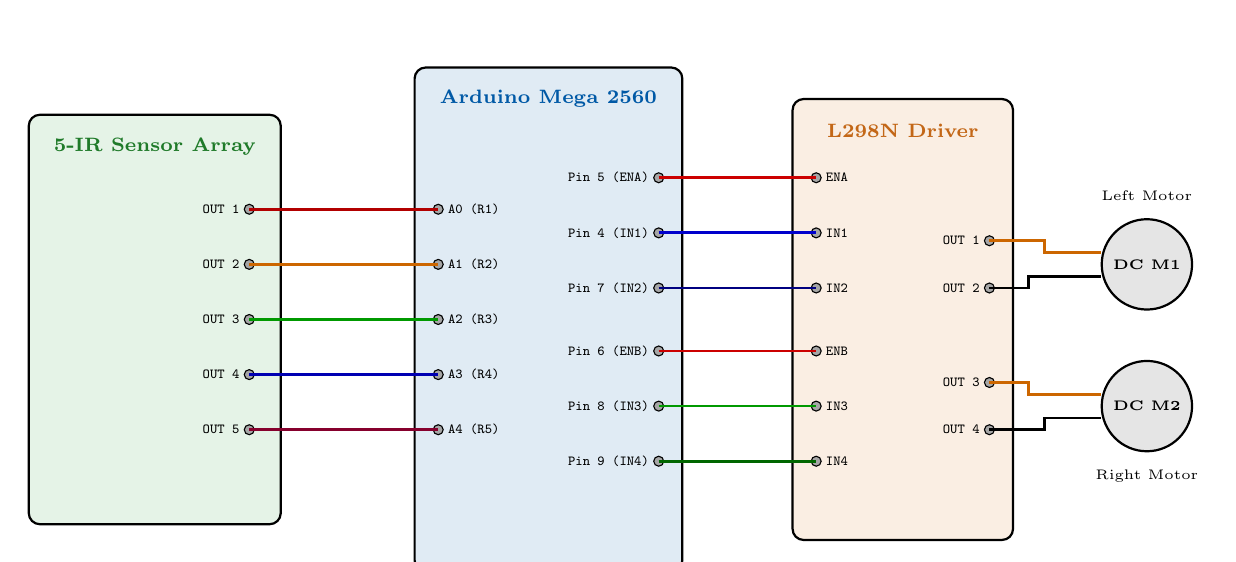
\begin{tikzpicture}[
    box/.style={draw=black, thick, rounded corners=4pt, fill=white, inner sep=5pt},
    pinlabel/.style={font=\ttfamily\tiny, text=black},
    wire/.style={line width=1.0pt}
]
    % 5-IR Sensor Array
    \node[box, fill=sensorgreen!12, minimum width=3.2cm, minimum height=5.2cm] (sensor) at (-5.0, 0) {};
    \node[font=\bfseries\scriptsize, text=sensorgreen!80!black] at (-5.0, 2.2) {5-IR Sensor Array};

    \node[pinlabel, anchor=east] (s_o1) at (-3.8, 1.4) {OUT 1};
    \node[pinlabel, anchor=east] (s_o2) at (-3.8, 0.7) {OUT 2};
    \node[pinlabel, anchor=east] (s_o3) at (-3.8, 0.0) {OUT 3};
    \node[pinlabel, anchor=east] (s_o4) at (-3.8, -0.7) {OUT 4};
    \node[pinlabel, anchor=east] (s_o5) at (-3.8, -1.4) {OUT 5};

    \foreach \p in {s_o1, s_o2, s_o3, s_o4, s_o5} {
        \filldraw[fill=gray!70, draw=black] (\p.east) circle (1.8pt);
    }

    % Arduino Mega 2560
    \node[box, fill=arduinoblue!12, minimum width=3.4cm, minimum height=6.4cm] (mega) at (0, 0) {};
    \node[font=\bfseries\scriptsize, text=arduinoblue] at (0, 2.8) {Arduino Mega 2560};

    % Left pins on Mega (Sensors)
    \node[pinlabel, anchor=west] (m_a0) at (-1.4, 1.4) {A0 (R1)};
    \node[pinlabel, anchor=west] (m_a1) at (-1.4, 0.7) {A1 (R2)};
    \node[pinlabel, anchor=west] (m_a2) at (-1.4, 0.0) {A2 (R3)};
    \node[pinlabel, anchor=west] (m_a3) at (-1.4, -0.7) {A3 (R4)};
    \node[pinlabel, anchor=west] (m_a4) at (-1.4, -1.4) {A4 (R5)};

    \foreach \p in {m_a0, m_a1, m_a2, m_a3, m_a4} {
        \filldraw[fill=gray!70, draw=black] (\p.west) circle (1.8pt);
    }

    % Right pins on Mega (Motor Driver Controls)
    \node[pinlabel, anchor=east] (m_p5) at (1.4, 1.8) {Pin 5 (ENA)};
    \node[pinlabel, anchor=east] (m_p4) at (1.4, 1.1) {Pin 4 (IN1)};
    \node[pinlabel, anchor=east] (m_p7) at (1.4, 0.4) {Pin 7 (IN2)};
    \node[pinlabel, anchor=east] (m_p6) at (1.4, -0.4) {Pin 6 (ENB)};
    \node[pinlabel, anchor=east] (m_p8) at (1.4, -1.1) {Pin 8 (IN3)};
    \node[pinlabel, anchor=east] (m_p9) at (1.4, -1.8) {Pin 9 (IN4)};

    \foreach \p in {m_p5, m_p4, m_p7, m_p6, m_p8, m_p9} {
        \filldraw[fill=gray!70, draw=black] (\p.east) circle (1.8pt);
    }

    % L298N Driver
    \node[box, fill=driverorange!12, minimum width=2.8cm, minimum height=5.6cm] (l298) at (4.5, 0) {};
    \node[font=\bfseries\scriptsize, text=driverorange!90!black] at (4.5, 2.4) {L298N Driver};

    % Left pins on L298N
    \node[pinlabel, anchor=west] (d_ena) at (3.4, 1.8) {ENA};
    \node[pinlabel, anchor=west] (d_in1) at (3.4, 1.1) {IN1};
    \node[pinlabel, anchor=west] (d_in2) at (3.4, 0.4) {IN2};
    \node[pinlabel, anchor=west] (d_enb) at (3.4, -0.4) {ENB};
    \node[pinlabel, anchor=west] (d_in3) at (3.4, -1.1) {IN3};
    \node[pinlabel, anchor=west] (d_in4) at (3.4, -1.8) {IN4};

    \foreach \p in {d_ena, d_in1, d_in2, d_enb, d_in3, d_in4} {
        \filldraw[fill=gray!70, draw=black] (\p.west) circle (1.8pt);
    }

    % Right pins on L298N (Motor outputs)
    \node[pinlabel, anchor=east] (d_out1) at (5.6, 1.0) {OUT 1};
    \node[pinlabel, anchor=east] (d_out2) at (5.6, 0.4) {OUT 2};
    \node[pinlabel, anchor=east] (d_out3) at (5.6, -0.8) {OUT 3};
    \node[pinlabel, anchor=east] (d_out4) at (5.6, -1.4) {OUT 4};

    \foreach \p in {d_out1, d_out2, d_out3, d_out4} {
        \filldraw[fill=gray!70, draw=black] (\p.east) circle (1.8pt);
    }

    % Motors
    \node[circle, draw=black, thick, fill=gray!20, minimum size=0.9cm, font=\tiny\bfseries] (m1) at (7.6, 0.7) {DC M1};
    \node[font=\tiny, above=0.1cm of m1] {Left Motor};

    \node[circle, draw=black, thick, fill=gray!20, minimum size=0.9cm, font=\tiny\bfseries] (m2) at (7.6, -1.1) {DC M2};
    \node[font=\tiny, below=0.1cm of m2] {Right Motor};

    % Wires: Sensor to Mega
    \draw[wire, color=red!70!black] (s_o1.east) -- (m_a0.west);
    \draw[wire, color=orange!80!black] (s_o2.east) -- (m_a1.west);
    \draw[wire, color=green!60!black] (s_o3.east) -- (m_a2.west);
    \draw[wire, color=blue!70!black] (s_o4.east) -- (m_a3.west);
    \draw[wire, color=purple!70!black] (s_o5.east) -- (m_a4.west);

    % Wires: Mega to L298N
    \draw[wire, color=red!80!black] (m_p5.east) -- (d_ena.west);
    \draw[wire, color=blue!80!black] (m_p4.east) -- (d_in1.west);
    \draw[wire, color=blue!50!black] (m_p7.east) -- (d_in2.west);
    \draw[wire, color=red!80!black] (m_p6.east) -- (d_enb.west);
    \draw[wire, color=green!60!black] (m_p8.east) -- (d_in3.west);
    \draw[wire, color=green!40!black] (m_p9.east) -- (d_in4.west);

    % Wires: L298N to Motors
    \draw[wire, color=orange!80!black] (d_out1.east) -- ++(0.7,0) |- ($(m1.west)+(0,0.15)$);
    \draw[wire, color=black] (d_out2.east) -- ++(0.5,0) |- ($(m1.west)+(0,-0.15)$);
    \draw[wire, color=orange!80!black] (d_out3.east) -- ++(0.5,0) |- ($(m2.west)+(0,0.15)$);
    \draw[wire, color=black] (d_out4.east) -- ++(0.7,0) |- ($(m2.west)+(0,-0.15)$);

\end{tikzpicture}
\caption{Circuit schematic of the line follower robot system.}
\label{fig_wiring}
\end{figure}

The connections shown in Figure~\ref{fig_wiring} establish signal routing and power distribution across the robotic system. The five optical outputs from the tracker board route to analog inputs A0 through A4 on the Arduino Mega 2560. Pulse width modulation pins 5 and 6 connect to the enable pins ENA and ENB of the L298N module to provide motor speed regulation. Digital pins 4, 7, 8, and 9 connect to inputs IN1 through IN4 to manage directional rotation. Output channels OUT1 and OUT2 energize the left motor, while channels OUT3 and OUT4 drive the right motor.

%--------------------------- Section 3 ---------------------------------
\section{Logic Used and System Flowchart}
The line following strategy uses five sensing points arranged symmetrically across the forward heading of the mobile platform. Sensor S1 occupies the far-left position, sensor S2 is on the inner left, sensor S3 occupies the true center, sensor S4 is on the inner right, and sensor S5 occupies the far-right position.

When a sensor hovers over the white floor, light reflects into the phototransistor, producing a low state of zero. When a sensor encounters the black trajectory, the light is absorbed, causing the sensor output to transition to a high state of one. The microcontroller samples all five inputs and determines the position of the line relative to the vehicle heading.

\subsection{System Flowchart}
Figure~\ref{fig_flowchart} shows the execution flow and decision branches governing the line follower robot.

\begin{figure}[H]
\centering
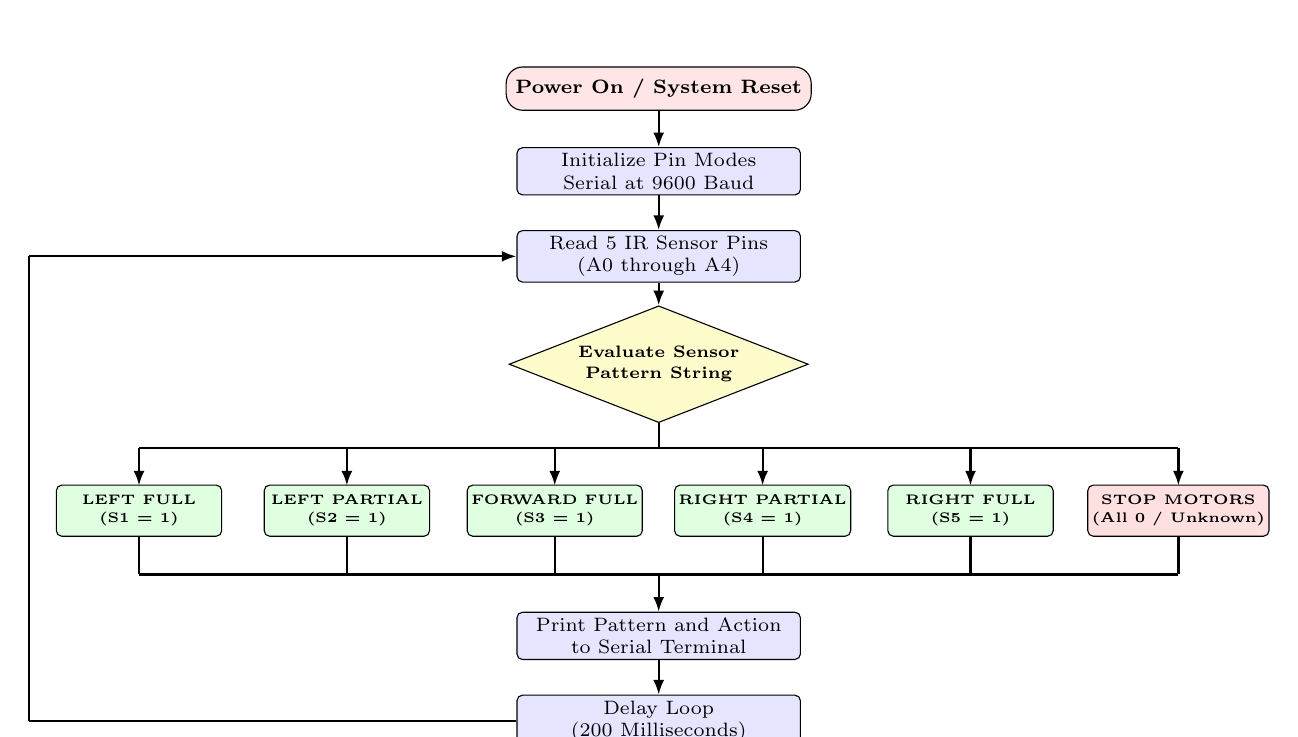
\begin{tikzpicture}[
    startstop/.style={rectangle, rounded corners=6pt, minimum width=3.4cm, minimum height=0.55cm, text centered, draw=black, fill=red!10, font=\scriptsize\bfseries},
    process/.style={rectangle, rounded corners=2pt, minimum width=3.6cm, minimum height=0.60cm, text centered, draw=black, fill=blue!10, font=\scriptsize, align=center, inner sep=2pt},
    decision/.style={diamond, aspect=2.2, minimum width=3.8cm, minimum height=0.90cm, text centered, draw=black, fill=yellow!20, font=\fontsize{6.5}{7.5}\selectfont\bfseries, align=center, inner sep=1pt},
    actionbox/.style={rectangle, rounded corners=2pt, minimum width=2.10cm, minimum height=0.65cm, text centered, draw=black, fill=green!12, font=\fontsize{5.5}{6.5}\selectfont\bfseries, align=center, inner sep=1.5pt},
    stopbox/.style={rectangle, rounded corners=2pt, minimum width=2.10cm, minimum height=0.65cm, text centered, draw=black, fill=red!12, font=\fontsize{5.5}{6.5}\selectfont\bfseries, align=center, inner sep=1.5pt},
    arrow/.style={thick, -{Latex[scale=0.8]}},
    line/.style={thick}
]
    \node[startstop] (start) at (0, 5.80) {Power On / System Reset};
    \node[process] (init) at (0, 4.75) {Initialize Pin Modes\\Serial at 9600 Baud};
    \node[process] (read) at (0, 3.67) {Read 5 IR Sensor Pins\\(A0 through A4)};
    \node[decision] (eval) at (0, 2.30) {Evaluate Sensor\\Pattern String};

    % 6 Action boxes across one horizontal row with clear 5.4mm gaps
    \node[actionbox] (b_lfull) at (-6.60, 0.44) {LEFT FULL\\(S1 = 1)};
    \node[actionbox] (b_lpart) at (-3.96, 0.44) {LEFT PARTIAL\\(S2 = 1)};
    \node[actionbox] (b_fwd)   at (-1.32, 0.44) {FORWARD FULL\\(S3 = 1)};
    \node[actionbox] (b_rpart) at ( 1.32, 0.44) {RIGHT PARTIAL\\(S4 = 1)};
    \node[actionbox] (b_rfull) at ( 3.96, 0.44) {RIGHT FULL\\(S5 = 1)};
    \node[stopbox]   (b_stop)  at ( 6.60, 0.44) {STOP MOTORS\\(All 0 / Unknown)};

    % Bottom blocks with clear 4.8mm vertical separation
    \node[process] (serial) at (0, -1.15) {Print Pattern and Action\\to Serial Terminal};
    \node[process] (delay)  at (0, -2.23) {Delay Loop\\(200 Milliseconds)};

    % Connect top with clearly visible arrows
    \draw[arrow] (start) -- (init);
    \draw[arrow] (init) -- (read);
    \draw[arrow] (read.south) -- (eval.north);

    % Distribution bus from eval with 4.8mm stem and arrows
    \draw[line] (eval.south) -- (0, 1.24);
    \draw[line] (-6.60, 1.24) -- (6.60, 1.24);
    \foreach \x in {-6.60, -3.96, -1.32, 1.32, 3.96, 6.60} {
        \draw[arrow] (\x, 1.24) -- (\x, 0.76);
    }

    % Collection bus to serial with 4.8mm connectors
    \draw[line] (-6.60, -0.37) -- (6.60, -0.37);
    \foreach \x in {-6.60, -3.96, -1.32, 1.32, 3.96, 6.60} {
        \draw[line] (\x, 0.11) -- (\x, -0.37);
    }
    \draw[arrow] (0, -0.37) -- (serial.north);

    % Connect bottom with clear 4.8mm arrow
    \draw[arrow] (serial) -- (delay);

    % Loop back
    \draw[line] (delay.west) -- (-8.0, -2.23);
    \draw[line] (-8.0, -2.23) -- (-8.0, 3.67);
    \draw[arrow] (-8.0, 3.67) -- (read.west);

\end{tikzpicture}
\caption{Flow diagram of the five-channel line tracking logic.}
\label{fig_flowchart}
\end{figure}

\subsection{Algorithmic Structure or Pseudocode}
Algorithm~\ref{algo_ir} details the sequential execution implemented in the firmware.

\begin{algorithm}[H]
\small
\SetAlFnt{\small}
\SetAlCapFnt{\small}
\SetAlCapNameFnt{\small}
\setlength{\algomargin}{1.2em}
\SetAlgoSkip{small}
\DontPrintSemicolon
\caption{Decision algorithm for five-channel line tracking}
\label{algo_ir}
Initialize serial communication at 9600 baud rate \\
Configure analog pins A0 through A4 as digital inputs \\
\BlankLine
\While{true}{
    Read digital input from pin A0 into variable s1 \\
    Read digital input from pin A1 into variable s2 \\
    Read digital input from pin A2 into variable s3 \\
    Read digital input from pin A3 into variable s4 \\
    Read digital input from pin A4 into variable s5 \\
    Transmit all sensor values over the serial interface \\
    \BlankLine
    \uIf{s1 == 0 and s2 == 0 and s3 == 0 and s4 == 0 and s5 == 0}{
        Print motor stop command
    }
    \uElseIf{s3 == 1 and s2 == 0 and s4 == 0}{
        Print forward full speed command
    }
    \uElseIf{s1 == 1}{
        Print turn left full speed command
    }
    \uElseIf{s2 == 1}{
        Print turn left partial speed command
    }
    \uElseIf{s5 == 1}{
        Print turn right full speed command
    }
    \uElseIf{s4 == 1}{
        Print turn right partial speed command
    }
    \Else{
        Print unknown state command
    }
    \BlankLine
    Wait for two hundred milliseconds \\
}
\end{algorithm}

%--------------------------- Section 4 ---------------------------------
\section{Code}
The Arduino C++ implementation loaded onto the microcontroller board is given below.

\begin{lstlisting}
#define S1 A0
#define S2 A1
#define S3 A2
#define S4 A3
#define S5 A4

void setup() {

  Serial.begin(9600);

  pinMode(S1, INPUT);
  pinMode(S2, INPUT);
  pinMode(S3, INPUT);
  pinMode(S4, INPUT);
  pinMode(S5, INPUT);
}

void loop() {

  int s1 = digitalRead(S1);
  int s2 = digitalRead(S2);
  int s3 = digitalRead(S3);
  int s4 = digitalRead(S4);
  int s5 = digitalRead(S5);

  // ------------------------------------
  // PRINT SENSOR VALUES
  // ------------------------------------

  Serial.print("Sensors: ");

  Serial.print(s1);
  Serial.print(" ");

  Serial.print(s2);
  Serial.print(" ");

  Serial.print(s3);
  Serial.print(" ");

  Serial.print(s4);
  Serial.print(" ");

  Serial.println(s5);


  // ------------------------------------
  // DECISION LOGIC
  // ------------------------------------

  // ALL WHITE
  if (s1 == 0 &&
      s2 == 0 &&
      s3 == 0 &&
      s4 == 0 &&
      s5 == 0) {

    Serial.println("ACTION: STOP ALL MOTORS");
  }


  // CENTER OF LINE
  else if (s3 == 1 &&
           s2 == 0 &&
           s4 == 0) {

    Serial.println("ACTION: MOVE FORWARD - FULL SPEED");
  }


  // LEFT FULL TURN
  else if (s1 == 1) {

    Serial.println("ACTION: TURN LEFT - FULL SPEED");
  }


  // LEFT PARTIAL TURN
  else if (s2 == 1) {

    Serial.println("ACTION: TURN LEFT - PARTIAL SPEED");
  }


  // RIGHT FULL TURN
  else if (s5 == 1) {

    Serial.println("ACTION: TURN RIGHT - FULL SPEED");
  }


  // RIGHT PARTIAL TURN
  else if (s4 == 1) {

    Serial.println("ACTION: TURN RIGHT - PARTIAL SPEED");
  }


  else {

    Serial.println("ACTION: UNKNOWN");
  }

  Serial.println("-------------------------");

  delay(200);
}
\end{lstlisting}

\newpage
%--------------------------- Section 5 ---------------------------------
\section{Results}
The integrated line follower system was tested under experimental floor tracking conditions. The five optical sensors continuously recorded ground reflectance, and the decision algorithm determined the required motor control actions.

Figure~\ref{fig_results_ir} displays the real-time serial monitor output obtained from the Arduino Mega 2560 operating at 9600 baud rate. When all five infrared sensors observe the high-reflectance white ground, the binary pattern reads 0 0 0 0 0, and the controller issues the command to stop all motors. When the tracking path shifts towards the rightmost detector, sensor S5 reads 1, and the system executes a full-speed right turn command to restore vehicle alignment over the guide trajectory. The experimental output confirms stable detection, prompt state transitions, and reliable decision execution throughout runtime.

\begin{figure}[H]
\centering
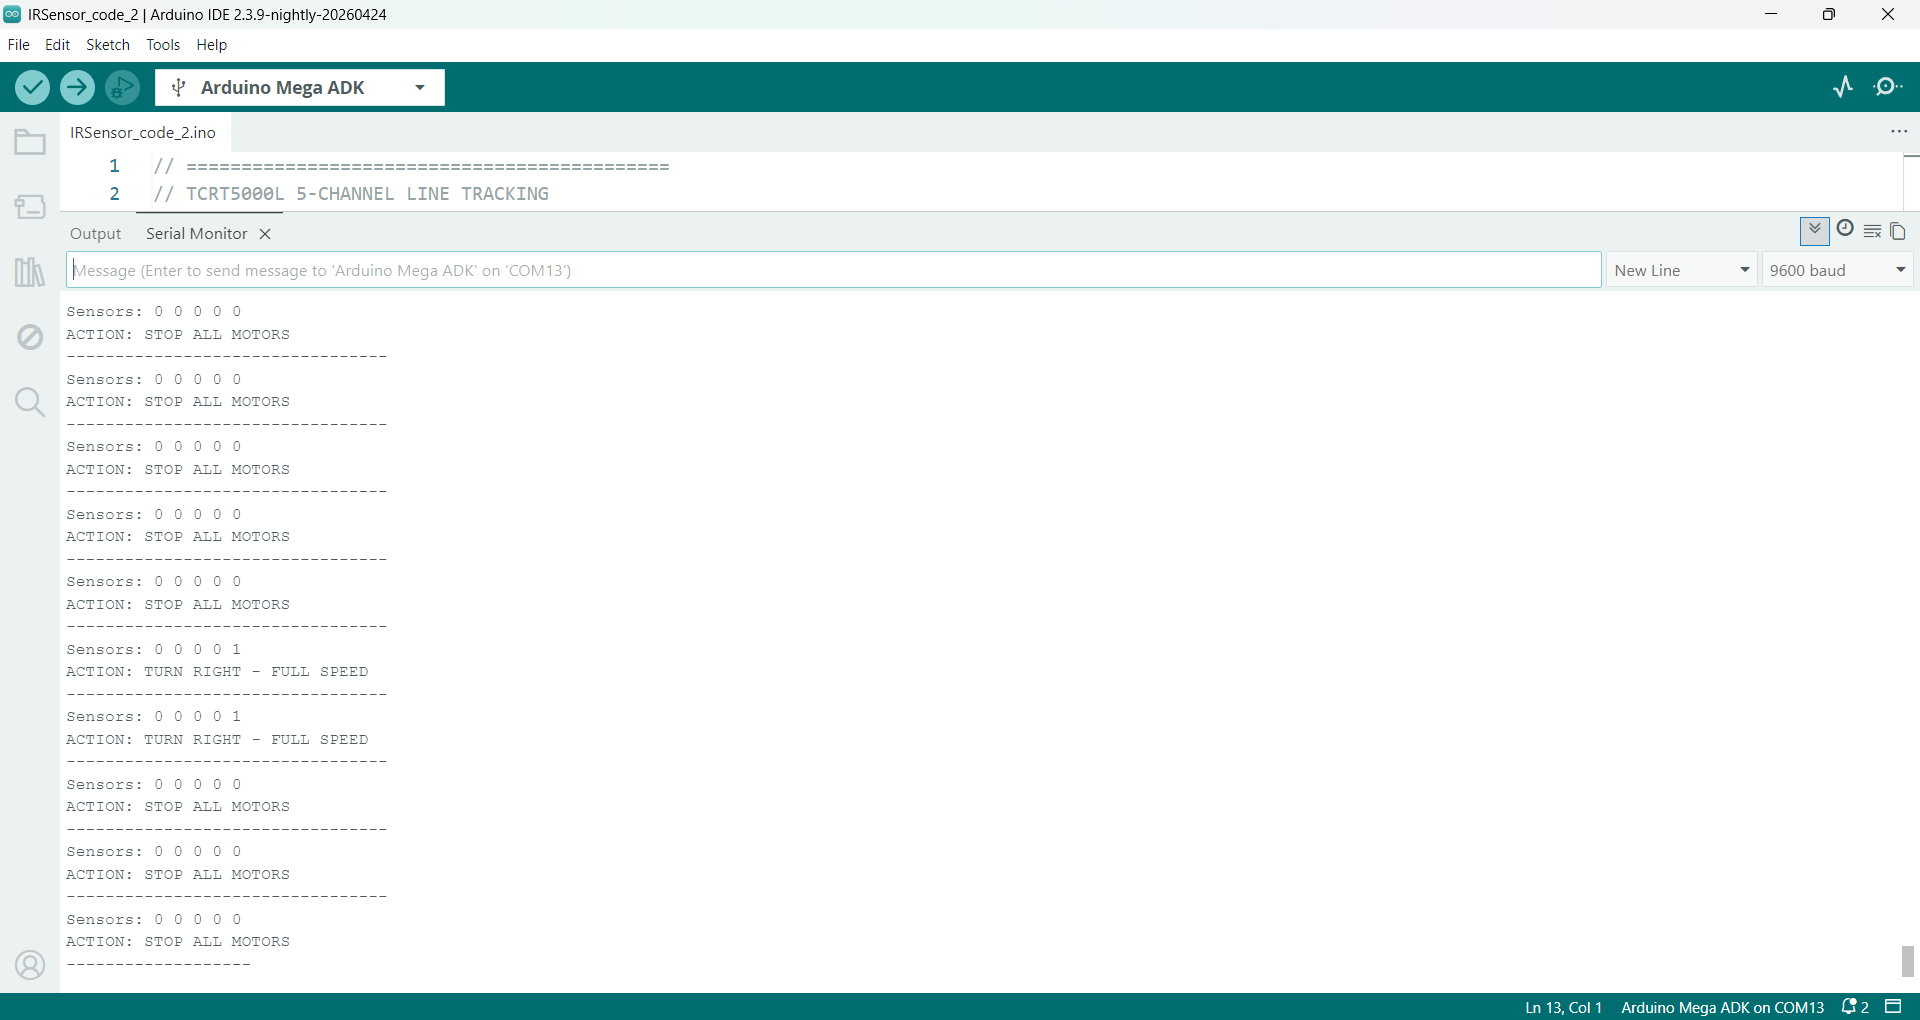
\includegraphics[width=0.72\linewidth]{IR.png}
\caption{Serial monitor output captured during the infrared tracking experiment.}
\label{fig_results_ir}
\end{figure}

%--------------------------- Section 6 ---------------------------------
\section{Video}
The recorded experimental demonstration verifying the operation of the five-channel infrared sensor system is hosted on the institutional repository.

\vspace{0.4cm}
\begin{center}
\href{https://indianinstituteofscience.sharepoint.com/:v:/s/MN2072026-27Aug-Dec/IQDZuwR3FS9WQohTNFhevTPpAUnHFneh8fEJVC7A9Jka7LE?e=B9qfHJ}{\large \textbf{Click Here to View the Infrared Sensor Demonstration Video}}
\end{center}

\vspace{0.4cm}
\noindent
The complete web link for manual browser access is provided below.

\vspace{0.2cm}
\noindent
{\footnotesize \url{https://indianinstituteofscience.sharepoint.com/:v:/s/MN2072026-27Aug-Dec/IQDZuwR3FS9WQohTNFhevTPpAUnHFneh8fEJVC7A9Jka7LE?e=B9qfHJ}}

\end{document}
